\documentclass[tikz,border=8pt]{standalone}
\usepackage{tikz}
\usetikzlibrary{arrows.meta,positioning}
\begin{document}
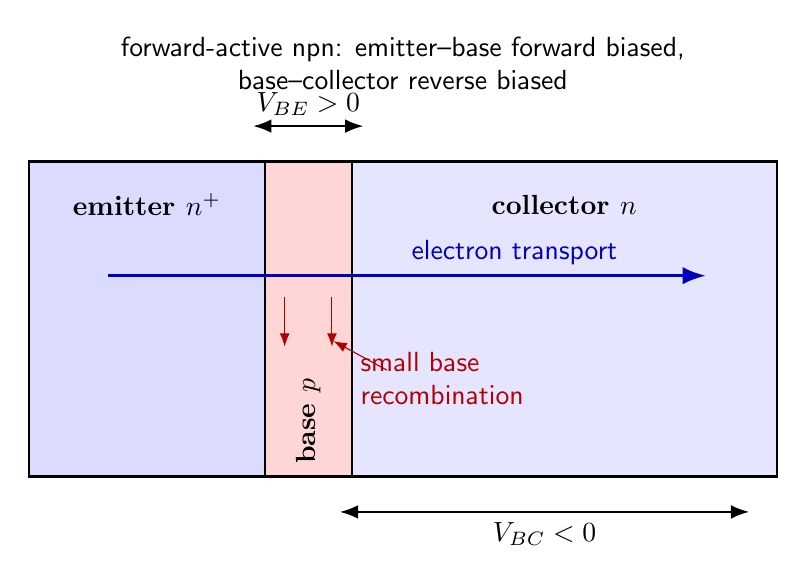
\begin{tikzpicture}[>=Latex,font=\sffamily]
  \fill[blue!14] (0,0) rectangle (3.0,4.0);
  \fill[red!16] (3.0,0) rectangle (4.1,4.0);
  \fill[blue!10] (4.1,0) rectangle (9.5,4.0);
  \draw[thick] (0,0) rectangle (9.5,4.0);
  \draw[thick] (3.0,0)--(3.0,4.0) (4.1,0)--(4.1,4.0);
  \node[font=\bfseries] at (1.5,3.45) {emitter $n^+$};
  \node[font=\bfseries,rotate=90] at (3.55,0.70) {base $p$};
  \node[font=\bfseries] at (6.8,3.45) {collector $n$};
  \draw[very thick,blue!75!black,->] (1.0,2.55)--(8.6,2.55)
    node[pos=0.68,above] {electron transport};
  \foreach \x in {3.25,3.85}
    \draw[red!70!black,->] (\x,2.28)--(\x,1.65);
  \node[align=left,red!70!black] at (5.25,1.25) {small base\\recombination};
  \draw[red!70!black,->] (4.55,1.35)--(3.87,1.72);
  \draw[<->,thick] (2.85,4.45)--node[above] {$V_{BE}>0$}(4.25,4.45);
  \draw[<->,thick] (3.95,-0.45)--node[below] {$V_{BC}<0$}(9.15,-0.45);
  \node[align=center] at (4.75,5.25)
    {forward-active npn: emitter--base forward biased,\\base--collector reverse biased};
\end{tikzpicture}
\end{document}
